\chapter{Methodology and Experimental Setup}\label{subseq:matrix-sets-and-hardware}

%Static solver configuration
\acrshort{athlet} is a CFD\footnote{Computational Fluid Dynamics} tool designed for computer-based simulations of transient thermo-hydraulic problems where topology of hydraulic circuits can be changed during a numerical simulation. As a direct consequence, the Jacobian matrix can frequently change with respect to both numerical values and the matrix sparsity structure between time integration steps. Since \acrshort{athlet} usually generates hundreds of matrices during a simulation, configuration of a linear solver in run-time becomes a time consuming and compute-expensive problem. Moreover, results of such dynamic solver configuration may be difficult to analyze and interpret.\\


In this study, a static solver configuration approach is used, instead. In other words, a solver is configured with only a small set of matrices, i.e. GRS matrix set, randomly saved during simulations of the most common \acrshort{grs} test scenarios. In the general case, it may lead to inaccurate conclusions, however, it is only one technically feasible approach.\\


Besides \acrshort{grs} matrix set, a second set was  used for verification of testing results. The set, called SuiteSparse matrix set, was generated by donwloading a dozen of matrices from SuiteSparse Matrix Collection \cite{sparse-matrix-collection:1}, \cite{sparse-matrix-collection:2} where we tried to pick out different matrices with respect to both the number of equations $n$ and matrix density i.e. ratio between the number of non-zero elements $nnz$ and the number of equations in a system.\\ 


The main matrix properties as well as matrix sparsity patterns are shown in Tables \ref{table:grs-matrix-set}, \ref{table:suite-sparse-matrix-set} and appendix \ref{app:sparsity-patterns}.\\


\begin{table}[!ht]
\small
\centering
\begin{tabular}{|c|c|c|c|c|c|}
\hline
Name     & \textit{n}       & \textit{nnz}      & \textit{nnz} / \textit{n} & \begin{tabular}[c]{@{}c@{}}Approximate\\ Condition\\  Number\end{tabular} & Structure     \\ \hline
pwr-3d   & 6009    & 32537    & 5.4147  & 1.019e+07                                                                 & SYMM-PTRN \\ \hline
cube-5   & 9325    & 117897   & 12.6431 & 1.592e+09                                                                 & SYMM-PTRN \\ \hline
cube-64  & 100657  & 1388993  & 13.7993 & 7.406e+08                                                                 & SYMM-PTRN \\ \hline
cube-645 & 1000045 & 13906057 & 13.9054 & 6.474e+08                                                                 & SYMM-PTRN \\ \hline
k3-2     & 130101  & 787997   & 6.0568  & 1.965e+15                                                                 & SYMM-PTRN \\ \hline
k3-18    & 1155955 & 7204723  & 6.2327  & 1.947e+12                                                                 & SYMM-PTRN \\ \hline
\end{tabular}
\caption[\acrshort{grs} matrix set]{ \acrshort{grs} matrix set, where SYMM - symmetric; NON-SYMM - non-symmetric; SYMM-PTRN- non-symmetric but with symmetric sparsity pattern}
\label{table:grs-matrix-set}
\end{table}




\begin{table}[!h]
\centering
\small
\begin{tabular}{|c|c|c|c|c|c|c|}
\hline
Name        & \textit{n}       & \textit{nnz}      & \textit{nnz} / \textit{n} & \begin{tabular}[c]{@{}c@{}}Approximate\\ Condition\\ Number\end{tabular} & Structure & Problem                                                      \\ \hline
cant        & 62451   & 4007383  & 64.1684 & 5.082e+05 & SYMM      & -                                                            \\ \hline
consph      & 83334   & 6010480  & 72.1251 & 2.438e+05 & SYMM      & -                                                            \\ \hline
CurlCurl\_3 & 1219574 & 13544618 & 11.1060 & 2.105e+05                                                                & SYMM      & \begin{tabular}[c]{@{}c@{}}Model\\ Reduction\end{tabular}    \\ \hline
Geo\_1438   & 1437960 & 63156690 & 43.9210 & 4.677e+05                                                                 & SYMM      & -                                                            \\ \hline
memchip     & 2707524 & 13343948 & 4.9285  & 1.305e+07                                                                & NON\_SYMM & \begin{tabular}[c]{@{}c@{}}Circuit\\ Simulation\end{tabular} \\ \hline
PFlow\_742  & 742793  & 37138461 & 49.9984 & 5.553e+06                                                                & SYMM      & -                                                            \\ \hline
pkustk10    & 80676   & 4308984  & 53.4110 & 5.589e+02 & SYMM      & Structural                                                   \\ \hline
torso3      & 259156  & 4429042  & 7.0903  & 2.456e+03                                                                      & NON\_SYMM & -                                                            \\ \hline
x104        & 108384  & 8713602  & 80.3956 & 3.124e+05 & SYMM      & Structural                                                   \\ \hline
\end{tabular}
\caption[SuiteSparse matrix set]{SuiteSparse matrix set, where SYMM - symmetric; NON-SYMM - non-symmetric; SYMM-PTRN- non-symmetric but with symmetric sparsity pattern}
\label{table:suite-sparse-matrix-set}
\end{table}

Approximations of condition numbers, shown in Tables \ref{table:grs-matrix-set} and \ref{table:suite-sparse-matrix-set},  were computed using the Rayleigh–Ritz procedure. The reader can become familiar with the procedure in \cite{rayleigh-ritz-procedure}. \acrshort{gmres} solver, configured with $1000$ iteration steps before the restart, was applied to un-preconditioned systems to generate a Krylov subspace for each matrix. Then, the resulting Hessenberg matrices were used for approximating eigenspaces and the corresponding eigenvalues. The approximations should be treated as lower bounds since the algorithm overestimates the smallest eigenvalues.\\


%The objective of this study is to find and configure a sparse linear solver which can fulfill all requirements listed above for the \acrshort{grs} matrix set. It is worth pointing out, as it was mentioned in section \ref{sec:athlet-overview}, \acrshort{athlet} performs many mathematical transformations upon the original system and, finally, generates an approximation of a Jacobian matrix. For that reason, one can assume that \acrshort{grs} matrix set can be structurally different from matrices coming naturally from finite-volume, finite-elements discretization or optimization problems. Therefore, SuiteSparse matrix set was used, from time to time, to examine this statement.\\


Two different hardware were available for this study. The first machine was a compute-cluster installed in \acrshort{grs} (\gls{hw1}) which was the main target. Additionally, \acrshort{lrz} CoolMUC-2 Linux cluster (\gls{hw2}) was used every time when some ambiguous results were obtained in order to check whether a problem was hardware, software or algorithmic specific. Table \ref{table:hardware-spec} shows compute-node specifications of both compute-clusters.\\


\begin{table}[!h]
\centering
\small
\begin{tabular}{|l|c|c|}
\hline
                    & HW1 (GRS) & HW2 (LRZ Linux) \\ \hline
Architecture        & x86\_64 & x86\_64 \\ \hline
CPU(s)              & 20 &  28 \\ \hline
On-line CPU(s) list & 0-19 &  0-27 \\ \hline
Thread(s) per core  & 1 &  1 \\  \hline
Core(s) per socket  & 10 & 14 \\ \hline
Socket(s)           & 2 &  2 \\ \hline
NUMA node(s)        & 2 &  4 \\ \hline
Model               & 62 &  63 \\ \hline
Model name          & E5-2680 v2 & 
E5-2697 v3 \\ \hline
Stepping            & 4 &  2 \\ \hline
CPU MHz             & 1200.0 &  2036.707 \\ \hline
Virtualization      & VT-x &  VT-x \\ \hline
L1d cache           & 32K &  32K \\ \hline
L1i cache           & 32K &  32K \\ \hline
L2 cache            & 256K &  256K \\ \hline
L3 cache            & 25600K &  17920K \\ \hline
NUMA node0 CPU(s)   & 0-9 &  0-6 \\ \hline
NUMA node1 CPU(s)   & 10-19 &  7-13 \\ \hline
NUMA node2 CPU(s)   & - &  14-20 \\ \hline
NUMA node3 CPU(s)   & - &  21-27 \\ \hline
RAM per node, GB   & 128 &  64 \\ \hline
\end{tabular}
\caption{Hardware specifications}
\label{table:hardware-spec}
\end{table}


For this study, OpenMPI implementation of the \acrshort{mpi} standard was used because of its open-source license and comprehensive documentation. The library has many options for processes pinning which was intensively used during the study.\\


To make process pinning explicit and deterministic, a Python script was developed to automatically generate rank-files based on the number of \acrshort{mpi} processes, \acrshort{openmp} threads per \acrshort{mpi} process, the maximum number of processing elements and the number of \acrshort{numa} domains. The scrip always leaves appropriate gaps between \acrshort{mpi} processes to allow each process to fork the corresponding number of threads within a parallel region.\\


\begin{figure}[!h]
\centering
	\begin{tabular}{cc}
			\subfloat[\textit{Spread} mode]{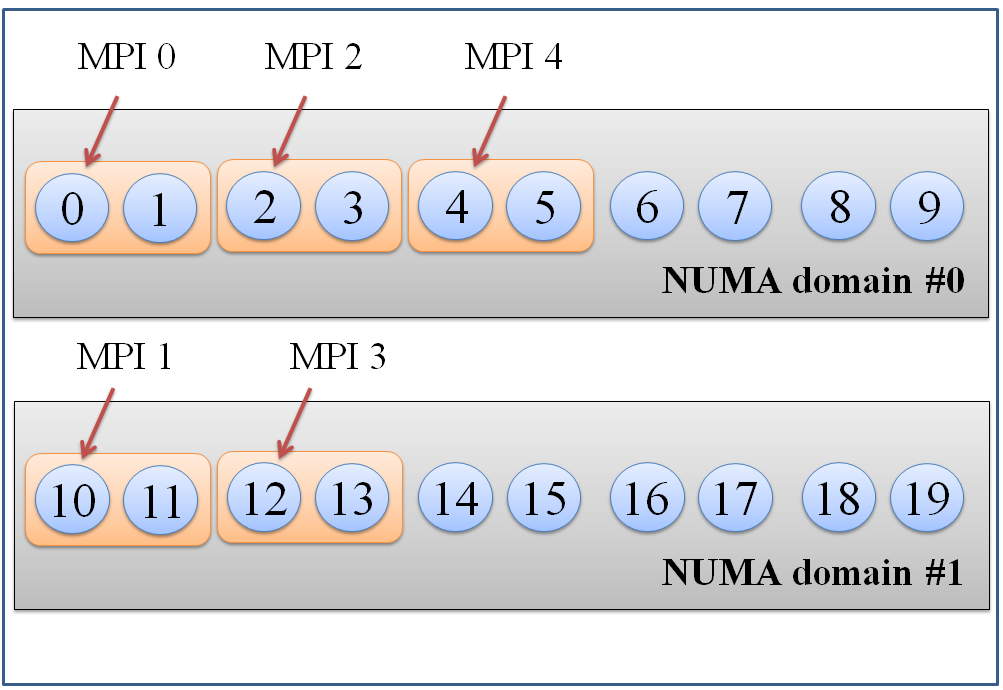
\includegraphics[width=0.45\textwidth]{figures/chapter-2/spread-mode.png}} &
		\subfloat[\textit{Close} mode]{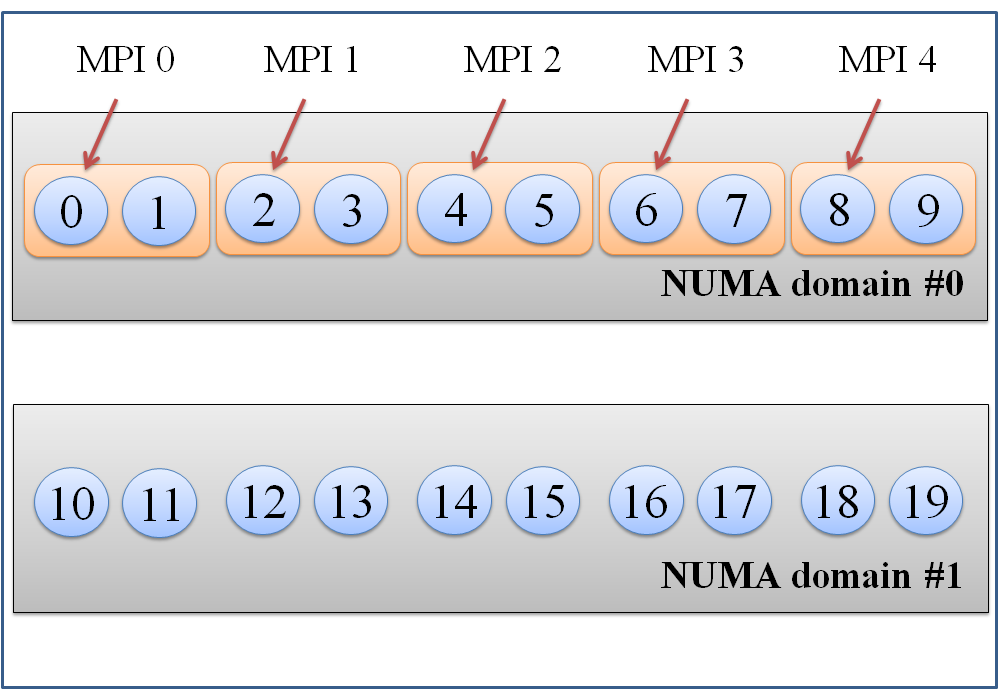
\includegraphics[width=0.45\textwidth]{figures/chapter-2/close-mode.png}} \\
	\end{tabular}
	\caption{An example of pinning 5 \acrshort{mpi} processes with 2 \acrshort{openmp} threads per process in case of \gls{hw1} hardware}
	\label{fig:python-script-rankfile-example}
\end{figure}


A rank-file specifies explicit mapping between \acrshort{mpi} processes, ranks, and actual processing elements, cores, of a compute-cluster. The script has two modes, namely: \textit{spread} and \textit{close}. Given a certain number of ranks, \textit{spread} mode tries to distribute them as spread as possible across multiple available \acrshort{numa} domains in a round-robin fashion. In contrast to \textit{spread} strategy, \textit{close} one groups ranks as close as possible to keep the maximum number of ranks within a single \acrshort{numa} domain. Figure \ref{fig:python-script-rankfile-example} shows an example of mapping 5 \acrshort{mpi} ranks and 2 \acrshort{openmp} threads per rank onto a compute node equipped with 20 cores and 2 \acrshort{numa} domains (\gls{hw1}).\\


In this study, \acrshort{petsc} 3.10 and OpenMPI 3.1.1 libraries were chosen and compiled with Intel 18.2 compiler.\\
